\setbeamercovered{transparent}

\begin{document}

% -------------------------------------------------------------------------------
% -------------------------------------------------------------------------------

\begin{frame}[plain]
  
\titlepage

\end{frame}

% -------------------------------------------------------------------------------
% -------------------------------------------------------------------------------

\subtitle[Outline]{Outline}

\begin{frame}{Outline}
    \begin{itemize}
        \item Motivation
        \item \epto{} explained
        \item \sys
        \item Evaluation
        \item Conclusion
    \end{itemize}
\end{frame}

\subtitle[Introduction]{Introduction}

\begin{frame}{Motivation}
    \epto{} was only evaluated using a \textbf{simulation}. 
    
    We need an evaluation with real peers to expose possible \textbf{limitations}.
\end{frame}

\begin{frame}{Motivation}
  \begin{itemize}
  \item Comparing \epto{} meant testing it against other algorithms
  \item No framework to easily deploy algorithms without having to rewrite them
  \end{itemize}

\end{frame}

\subtitle[Description]{Description}

\begin{frame}{What is \epto{}?}
	\textbf{Epidemic Total Order Algorithm:}
	\begin{itemize}
		\item Probabilistic dissemination algorithm
		\item Provides deterministic total order
		\item Scales in the number of peers and events
		\item Churn resistant
	\end{itemize}
\end{frame}

%\begin{frame}{What is \epto{}? (2)}
%	\textbf{Properties satisfied:}
%\begin{itemize}
%	\item Integrity
%	\item Validity
%	\item Total Order
%	\item Probabilistic Agreement
%\end{itemize}
%\end{frame}

%\begin{frame}{Properties satisfied}
%	\begin{itemize}
%		\item Integrity
%		\item Validity
%		\item Total Order
%		\item Probabilistic Agreement
%	\end{itemize}
%\end{frame}
\begin{frame}{\epto{} architecture}
    \begin{figure}
        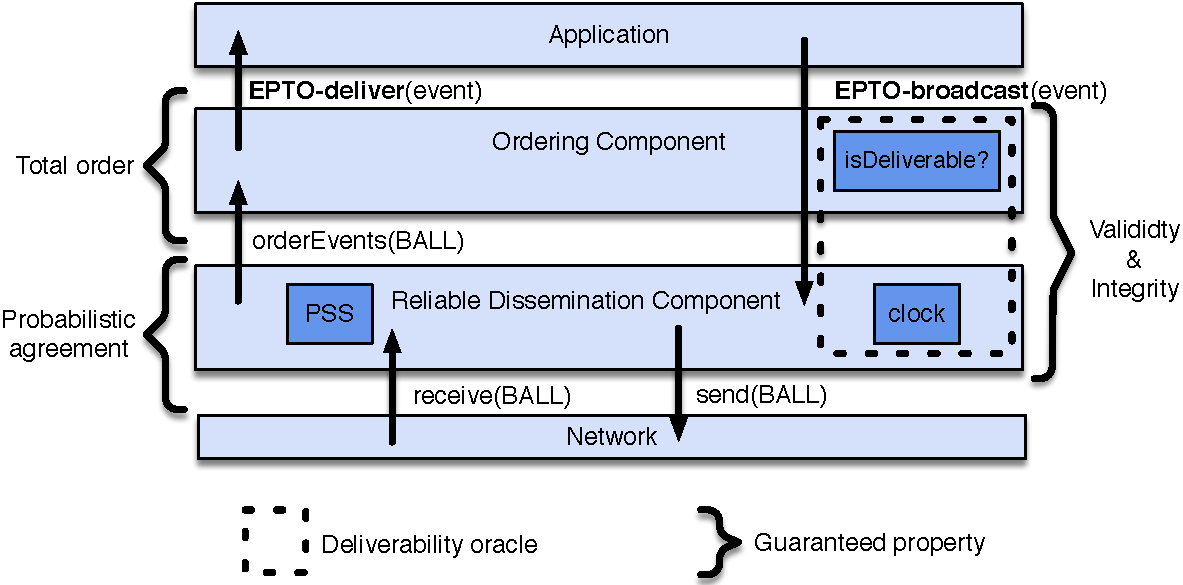
\includegraphics[scale=0.5]{figures/architecture}
    \end{figure}
\tiny{M. Matos, H. Mercier, P. Felber, R. Oliveira and J. Pereira, “EpTO: An epidemic total order algorithm for Large-scale distributed systems”, in Proceedings of the 16th Annual Middleware Conference, ACM, 2015, pp. 100–111.
}
\end{frame}

\begin{frame}{\sys{} features}
    \begin{itemize}
    	\item Compatible with any distributed algorithm provided it runs on Docker
    	\item support for a user-provided tracker
    	\item Automated benchmarking execution
    	\item Containers allow for more than 1 peer per physical node
    	\item Can simulate churn or follow real traces
    \end{itemize}
\end{frame}

\begin{frame}{\sys{} architecture}
	\begin{figure}
		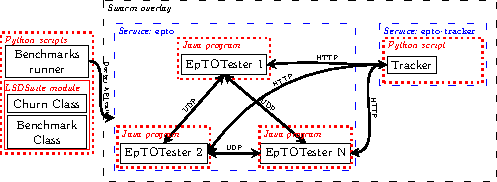
\includegraphics[scale=1.2]{complete-architecture}
	\end{figure}
\end{frame}

\begin{frame}{\sys{} Configuration and Logging}
	The protocol, churn and framework configuration is done through \textsc{YAML} files
	
	The protocols logs must be written in a file to be extracted to the host
\end{frame}

\subtitle[Evaluation]{Evaluation}

\begin{frame}{Evaluation}
    We evaluate \epto{} against \jgroups{} according scaling peers and global event throughput per second.
    
    We write $(n,e)$ where $n$ is the number of peers and $e$ is the global event throughput per second.
\end{frame}

\begin{frame}{Bandwidth}
	\begin{figure}
		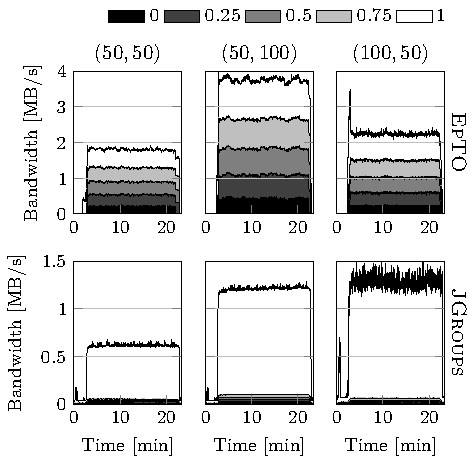
\includegraphics[scale=0.6]{bandwidth-nochurn}
	\end{figure}
\end{frame}

\begin{frame}{Bandwidth Synthetic Churn}
	\begin{figure}
		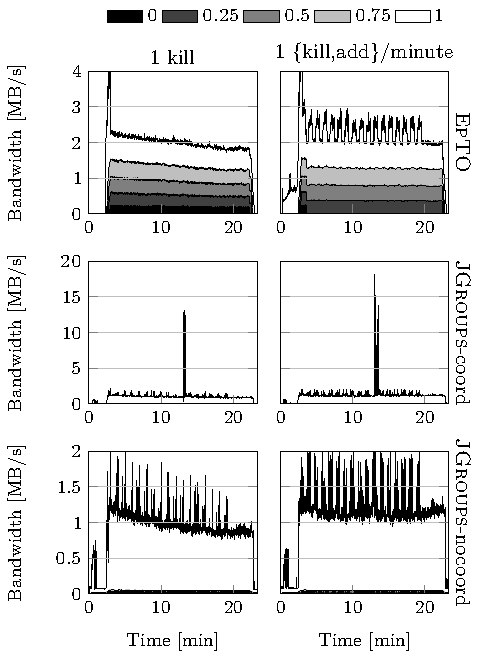
\includegraphics[scale=0.68]{bandwidth-synth-churn}
	\end{figure}
\end{frame}

\begin{frame}{Bandwidth Real Churn}
	\begin{figure}
		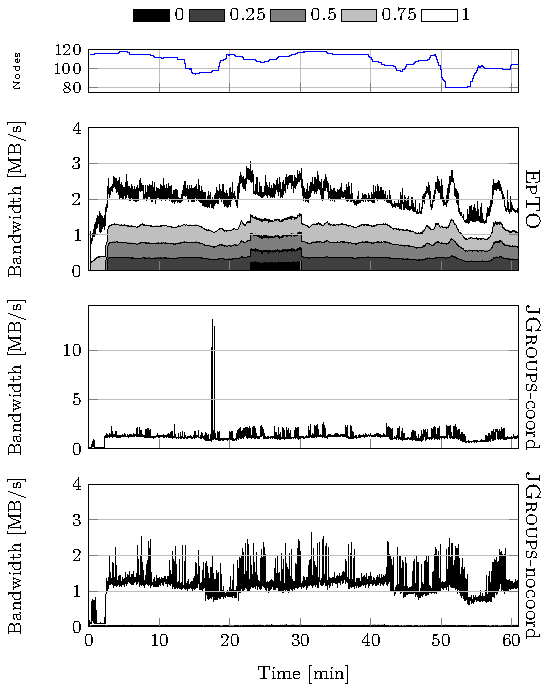
\includegraphics[scale=0.65]{bandwidth-real-churn}
	\end{figure}
\end{frame}

\begin{frame}{Local Dissemination Stretch}
	\begin{figure}
		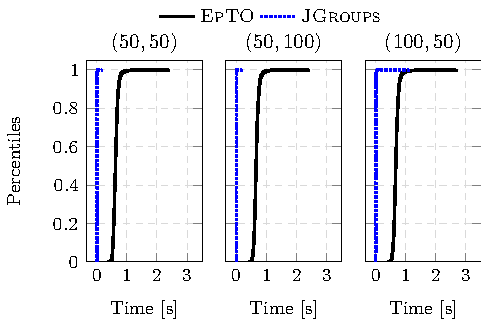
\includegraphics[scale=1]{local-diss-stretch-nochurn}
	\end{figure}
\end{frame}

\begin{frame}{Local Dissemination Stretch Synthetic Churn}
	\begin{figure}
		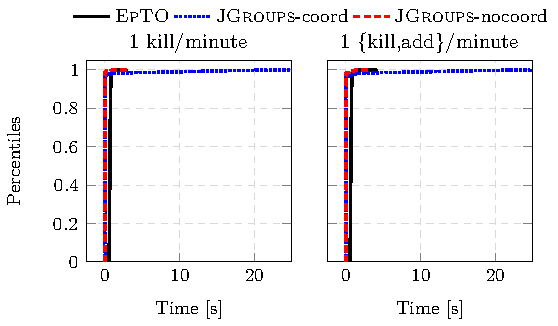
\includegraphics[scale=1]{local-diss-stretch-synth-churn}
	\end{figure}
\end{frame}

\begin{frame}{Local Dissemination Stretch Real Churn}
	\begin{figure}
		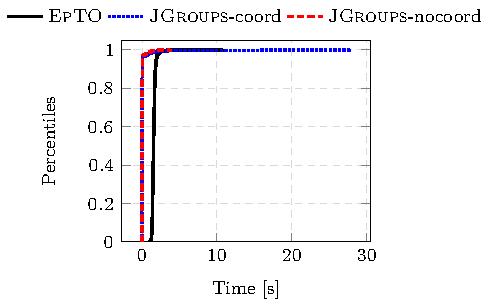
\includegraphics[scale=1]{local-diss-stretch-real-churn}
	\end{figure}
\end{frame}

\begin{frame}{Local Times}
	\begin{figure}
		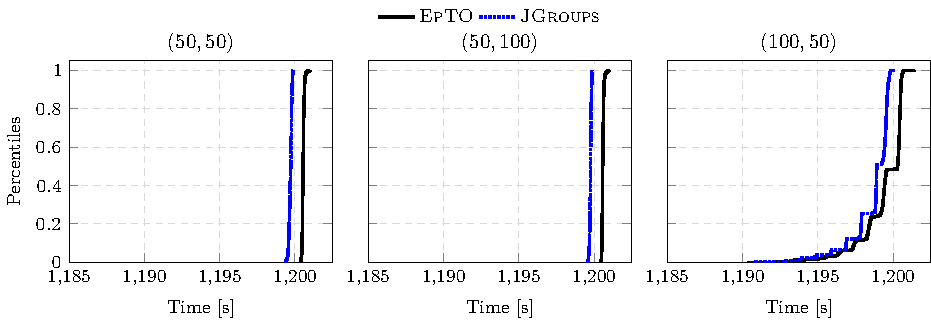
\includegraphics[scale=0.70]{local-times-nochurn}
	\end{figure}
\end{frame}

\begin{frame}{Local Times Synthetic Churn}
	\begin{figure}
		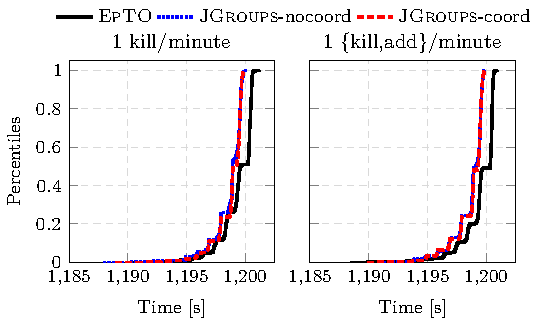
\includegraphics[scale=1]{local-times-synth-churn}
	\end{figure}
\end{frame}

\begin{frame}{Local Times Real Churn}
	\begin{figure}
		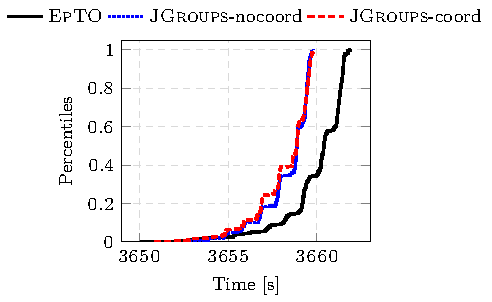
\includegraphics[scale=1]{local-times-real-churn}
	\end{figure}
\end{frame}

\begin{frame}{Global Times}
	\begin{figure}
		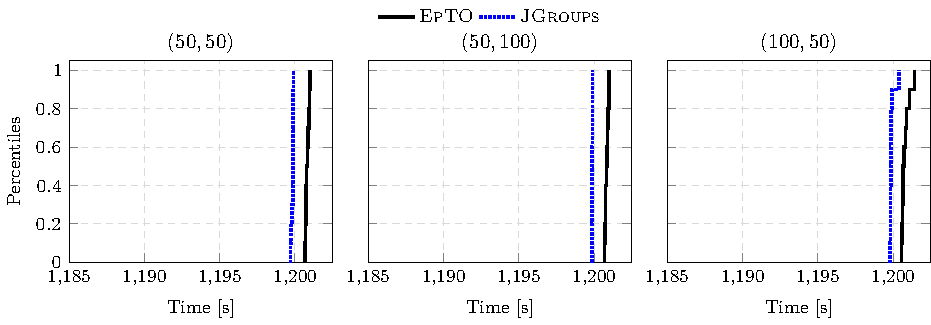
\includegraphics[scale=0.60]{global-times-nochurn}
	\end{figure}
\end{frame}

\begin{frame}{Global Times Synthetic Churn}
	\begin{figure}
		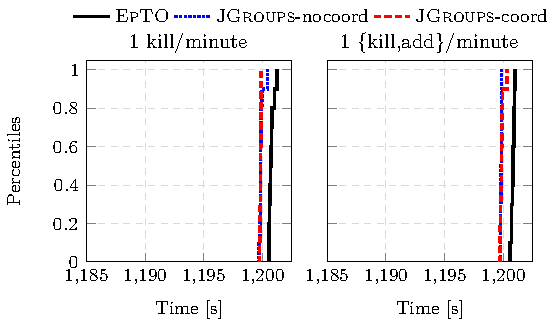
\includegraphics[scale=1]{global-times-synth-churn}
	\end{figure}
\end{frame}

\begin{frame}{Global Times Real Churn}
	\begin{figure}
		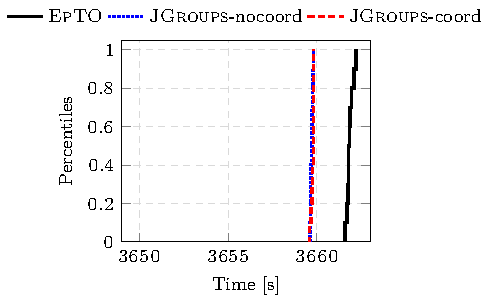
\includegraphics[scale=1]{global-times-real-churn}
	\end{figure}
\end{frame}

\subtitle[Conclusion]{Conclusion}

\begin{frame}{Future Work}
    \begin{itemize}
        \item Obtain more resources to have stronger results
        \item Implement a Push-Pull \epto{} version
        \item Use Kubernetes instead of Docker + Docker swarm
        \item Refine Framework Architecture
    \end{itemize}
\end{frame}

\begin{frame}[standout]
	Questions?
\end{frame}

% -------------------------------------------------------------------------------
% -------------------------------------------------------------------------------

\end{document}

% -------------------------------------------------------------------------------
